% Created 2018-04-09 Mon 07:42
% Intended LaTeX compiler: pdflatex
\documentclass[10pt]{beamer}
\usepackage[utf8]{inputenc}
\usepackage[T1]{fontenc}
\usepackage{graphicx}
\usepackage{grffile}
\usepackage{longtable}
\usepackage{wrapfig}
\usepackage{rotating}
\usepackage[normalem]{ulem}
\usepackage{amsmath}
\usepackage{textcomp}
\usepackage{amssymb}
\usepackage{capt-of}
\usepackage{hyperref}
\usetheme{Boadilla}
\author{ECON 420: Game Theory}
\date{Spring 2018}
\title{Sequential Games}
\usecolortheme{seagull}
\usefonttheme[onlylarge]{structurebold}
\usefonttheme[onlymath]{serif}
\setbeamerfont*{frametitle}{size=\normalsize,series=\bfseries}
\setbeamertemplate{navigation symbols}{}
\setbeamertemplate{itemize item}[triangle]
\setbeamertemplate{footline}{}
\setbeamertemplate{enumerate items}[default]
\hypersetup{
 pdfauthor={ECON 420: Game Theory},
 pdftitle={Sequential Games},
 pdfkeywords={},
 pdfsubject={},
 pdfcreator={Emacs 25.2.2 (Org mode 9.1.6)}, 
 pdflang={English}}
\begin{document}

\maketitle

\begin{frame}[label={sec:org310cba3}]{}
\alert{Centipede game}
\begin{enumerate}
\item 2 players play for 10 rounds
\item Each round another unit of payoff is added to the pot (starting with one unit)
\item Players alternate turns, choose to either:
\begin{itemize}
\item Stop, and collect the entire pot for themselves
\item Continue, one is added to the pot and next player chooses
\end{itemize}
\end{enumerate}
\end{frame}

\begin{frame}[label={sec:orgf146b48}]{}
\alert{Sequential games}
\begin{itemize}
\item Games where there is a strict order of play
\item Games where players take turns moving are sequential
\item Real-world games are generally combinations of sequential and simultaneous games
\end{itemize}
\end{frame}

\begin{frame}[label={sec:orgf5407a3}]{}
\alert{Game trees}
\begin{itemize}
\item We will visualize games using \alert{game trees}
\item Representing a game as a tree is known as the "extensive form" of a game
\item The tree shows all components of a game: players, actions and strategies, payoffs
\end{itemize}
\end{frame}

\begin{frame}[label={sec:org4f5838a}]{}
\alert{Nodes and branches}
\begin{itemize}
\item \emph{Nodes} are points on the tree where choices are made
\begin{itemize}
\item The first node is called the \emph{root node}
\item The last nodes (without branches) are \emph{terminal nodes}
\end{itemize}
\item \emph{Branches} show the actions available for the player to choose among at any node
\item A node (and its branches) represent a "turn" for a player
\item Payoffs are listed at the terminal nodes
\begin{itemize}
\item Each player in the game gets a payoff at each node
\item Remember: Higher numbers are always better
\end{itemize}
\end{itemize}
\end{frame}

\begin{frame}[label={sec:org9ad0a92}]{}
\alert{External uncertainty}
\begin{itemize}
\item With external uncertainty, we introduce nature as a "player"
\item Nature gets its own node, branches are possible outcomes
\item Players calculate expected payoffs across the possible outcomes of nature's "choice"
\end{itemize}
\end{frame}

\begin{frame}[label={sec:orgce36290}]{}
\begin{center}
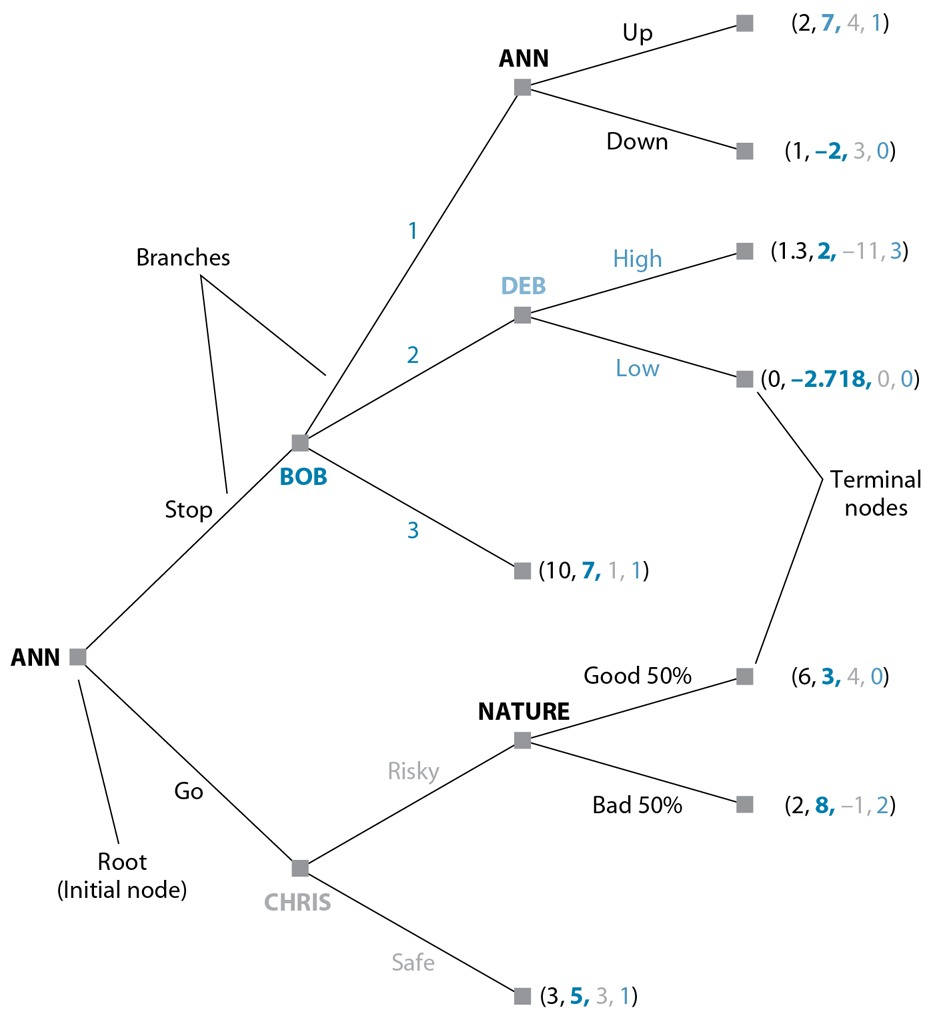
\includegraphics[height=\textheight]{./img/GAMES4_FIG03.01.jpg}
\end{center}
\end{frame}

\begin{frame}[label={sec:orgb8db8b7}]{}
\alert{Moves vs strategy}
\begin{itemize}
\item A choice of action at a node is called a \emph{move}
\item A strategy is a \emph{complete plan of action}
\begin{itemize}
\item A set of moves that will be performed if a certain situation arises
\item Strategies are collections of statements like "if \emph{X} then \emph{Y}" for \emph{any possible X}
\end{itemize}
\end{itemize}
\end{frame}

\begin{frame}[label={sec:orgcc19ba1}]{}
\alert{Example}
\begin{itemize}
\item How many strategies does Ann have?
\item What are they?
\end{itemize}
\end{frame}

\begin{frame}[label={sec:orgf48d68d}]{}
\alert{Strategies}
\begin{itemize}
\item Strategies must include actions at \emph{each node where a player can move}
\item This includes the nodes that won't be reached if a player chooses a particular set of actions
\item This is because hypothetical moves might help determine which moves should be chosen at earlier nodes
\item Choices early in a game are affected by \emph{expectations} about what will happen later in the game
\end{itemize}
\end{frame}

\begin{frame}[label={sec:orge524e7b}]{}
\alert{Finding equilibria in game trees}
\begin{itemize}
\item Consider one person's decision tree (is this a game?)
\item The player (Carmen) is considering whether or not to start smoking
\item Carmen first decides whether to start, then decides whether to continue
\item What should Carmen do?
\end{itemize}
\end{frame}

\begin{frame}[label={sec:org10f6f58}]{}
\begin{center}
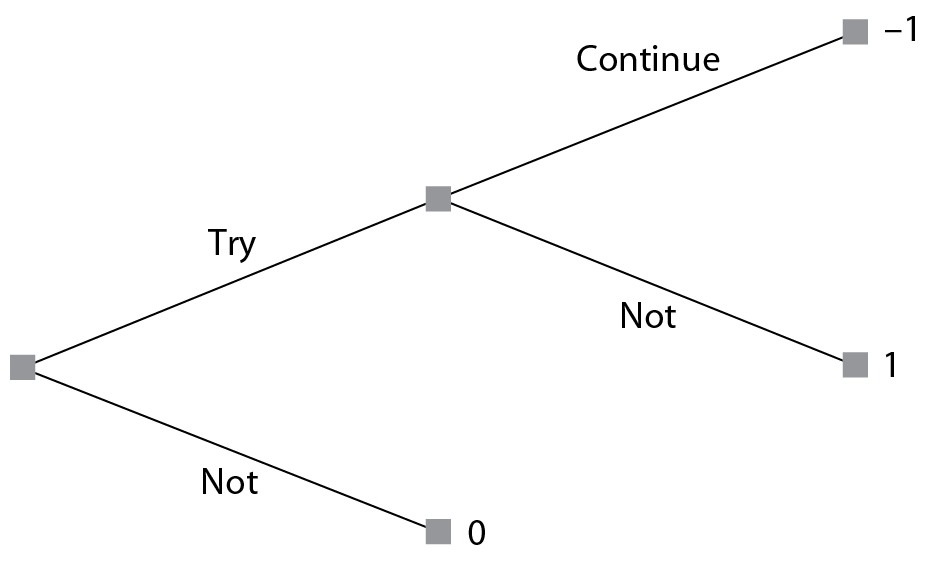
\includegraphics[width=0.75\textwidth]{./img/GAMES4_FIG03.02.jpg}
\end{center}
\end{frame}

\begin{frame}[label={sec:orgd8673fa}]{}
\alert{A decision tree as a game}
\begin{itemize}
\item Previous decision tree ignore that Carmen may become addicted if she starts smoking
\begin{itemize}
\item Once addicted, quitting becomes worse (payoffs are lower)
\end{itemize}
\item Carmen knows she may become addicted and that her payoffs might change if she starts smoking
\item We can think of this as a game where the players are Carmen today and Carmen in the future (after the initial decision is made)
\item Today's Carmen and future Carmen have different payoffs
\end{itemize}
\end{frame}

\begin{frame}[label={sec:org792c1c4}]{}
\begin{center}
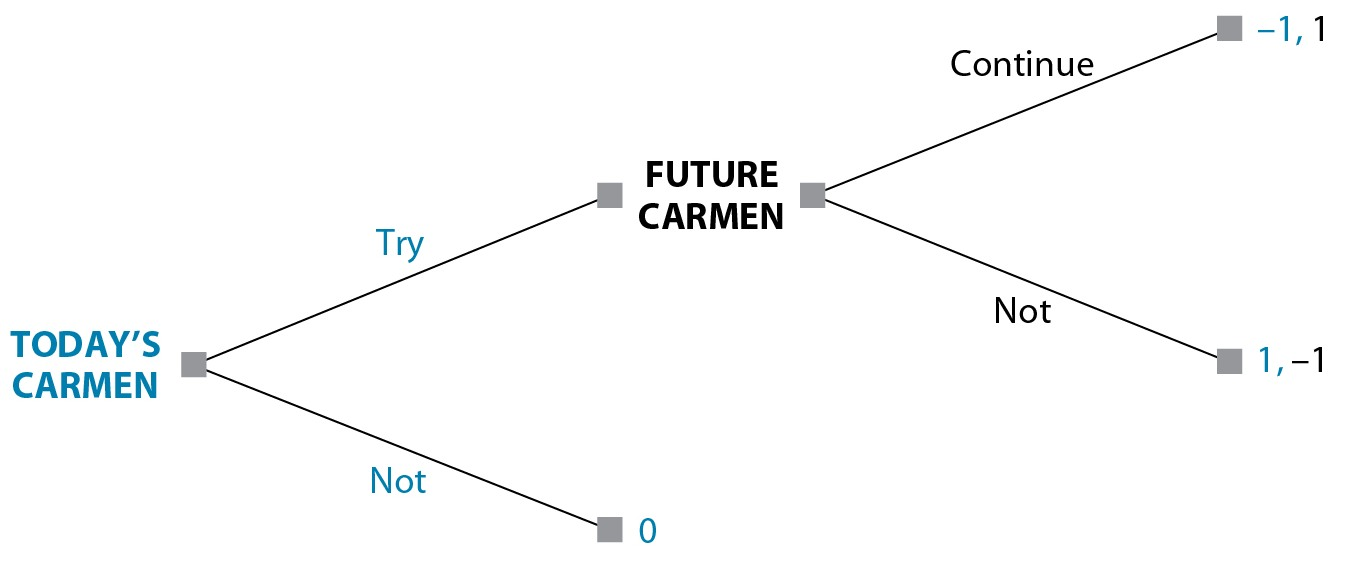
\includegraphics[width=0.75\textwidth]{./img/GAMES4_FIG03.03.jpg}
\end{center}
\end{frame}

\begin{frame}[label={sec:org1cbdef0}]{}
\alert{Pruning}
\begin{itemize}
\item Starting at the end, we can "prune" the branches that we know will not be chosen
\item When there is one action remaining at the final nodes, this means that the "final" decision moves back to the previous node (rollback)
\item Starting at the end and moving backward by pruning allows today's Carmen to choose the best option for herself
\item When all players use rollback analysis, the result of the game is called a \emph{rollback equilibrium}
\end{itemize}
\end{frame}

\begin{frame}[label={sec:org0c8b008}]{}
\alert{Smoking game}
\begin{itemize}
\item What are the rollback equilibrium strategies?
\item Can either player do better by changing their strategies?
\end{itemize}
\end{frame}

\begin{frame}[label={sec:orge5b4132}]{}
\begin{center}
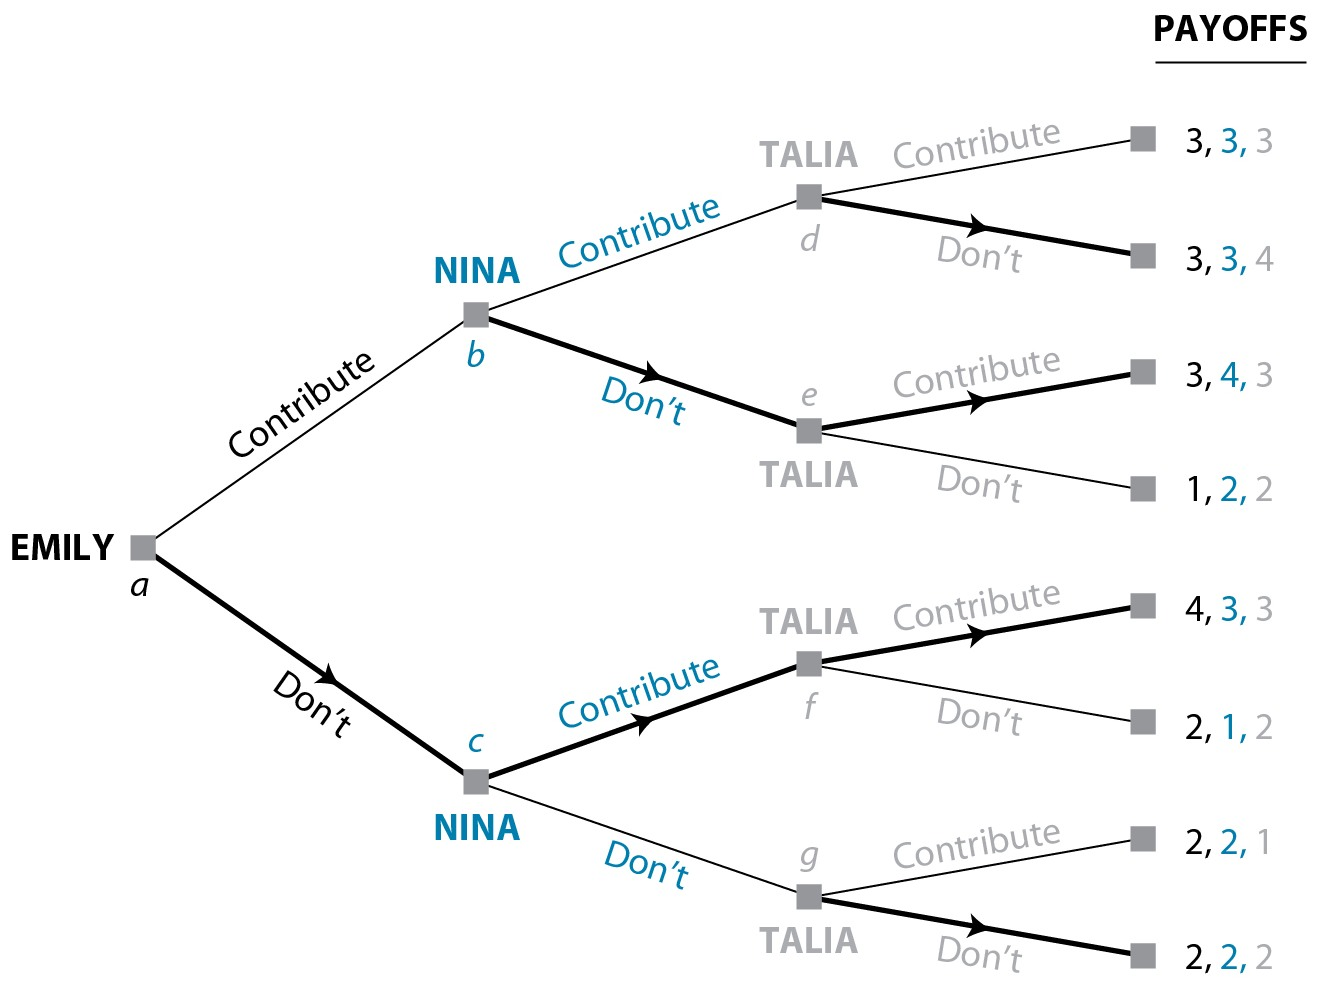
\includegraphics[width=0.75\textwidth]{./img/GAMES4_FIG03.06.jpg}
\end{center}
\end{frame}

\begin{frame}[label={sec:orgc7f0b27}]{}
\alert{Three-player game}
\begin{itemize}
\item How many strategies does each player have?
\item What is the rollback equilibrium?
\item What are the rollback equilibrium strategies?
\end{itemize}
\end{frame}

\begin{frame}[label={sec:orgcf7ed20}]{}
\alert{Example: Ultimatum game}
\begin{itemize}
\item Player 1:
\begin{itemize}
\item Choose how to split 10 units so that both players get at least one unit
\end{itemize}
\item Player 2:
\begin{itemize}
\item Choose to either:
\begin{enumerate}
\item Accept the split (you get what player 1 chooses for you)
\item Reject the split (neither player gets anything)
\end{enumerate}
\end{itemize}
\end{itemize}
\end{frame}

\begin{frame}[label={sec:orgb73dc76}]{}
\alert{Example: Centipede game}
\begin{itemize}
\item What does the game tree look like?
\item What are the strategies for each player?
\item What is the rollback equilibrium outcome?
\item What are the rollback equilibrium strategies?
\item Is this the outcome we observe in practice?
\end{itemize}
\end{frame}

\begin{frame}[label={sec:orgb0d06de}]{}
\alert{Limitations of rollback analysis} 
\begin{itemize}
\item Simple games can become difficult to express in extensive form 
\begin{itemize}
\item How many moves does the first player have in tic-tac-toe?
\item How many moves does the second player have?
\end{itemize}
\item Some sequential games are \emph{impossible} to express in extensive form!
\end{itemize}
\end{frame}

\begin{frame}[label={sec:orgd4d9770}]{}
\begin{center}
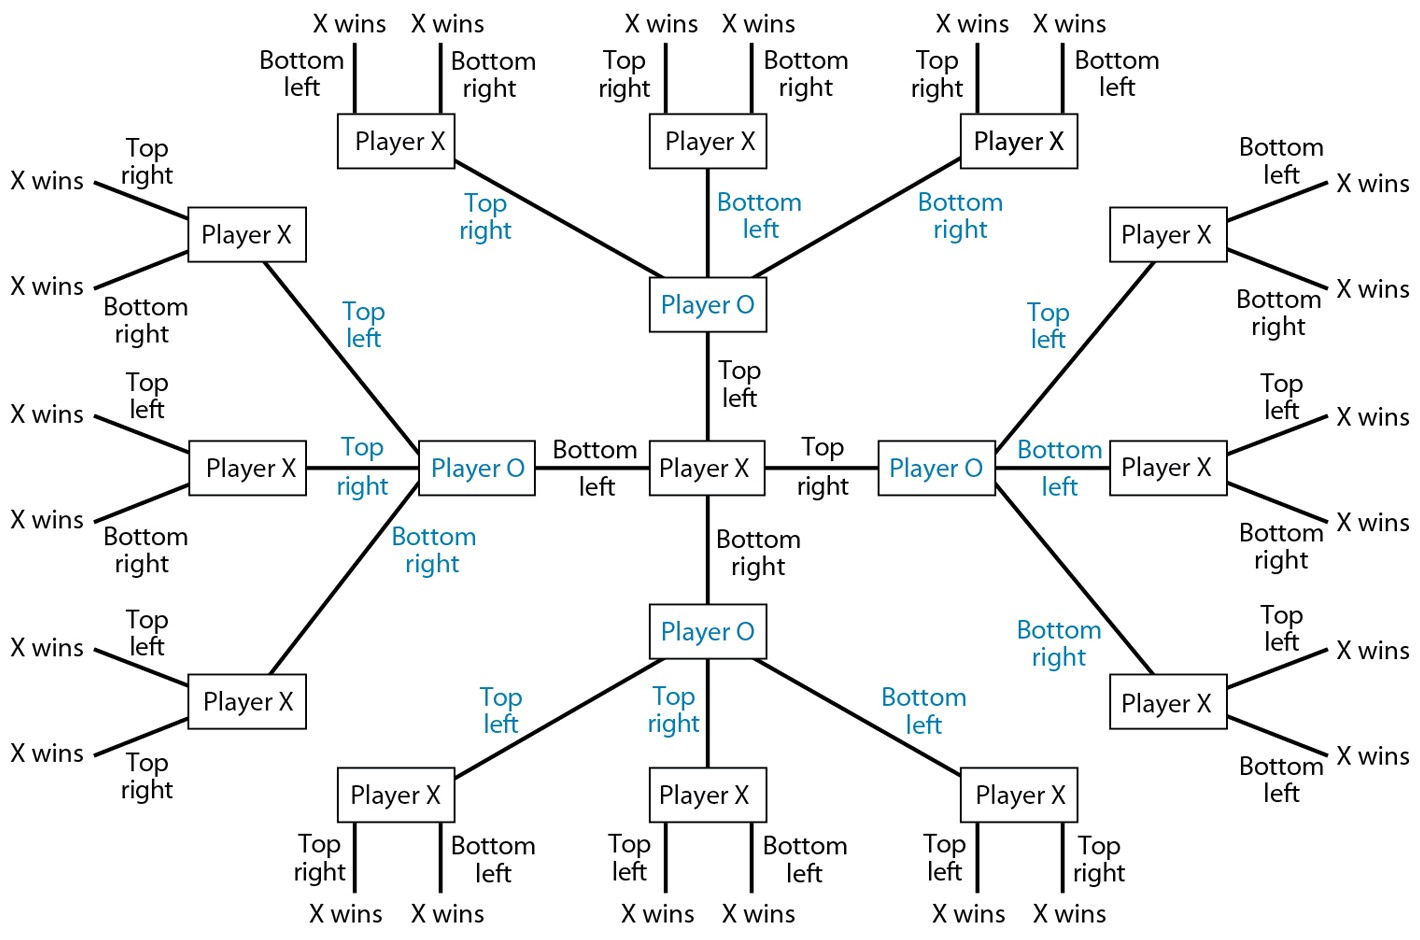
\includegraphics[width=.75\textwidth]{./img/GAMES4_FIG03.07.jpg}
\end{center}
\end{frame}

\begin{frame}[label={sec:org0c475f3}]{}
\begin{center}
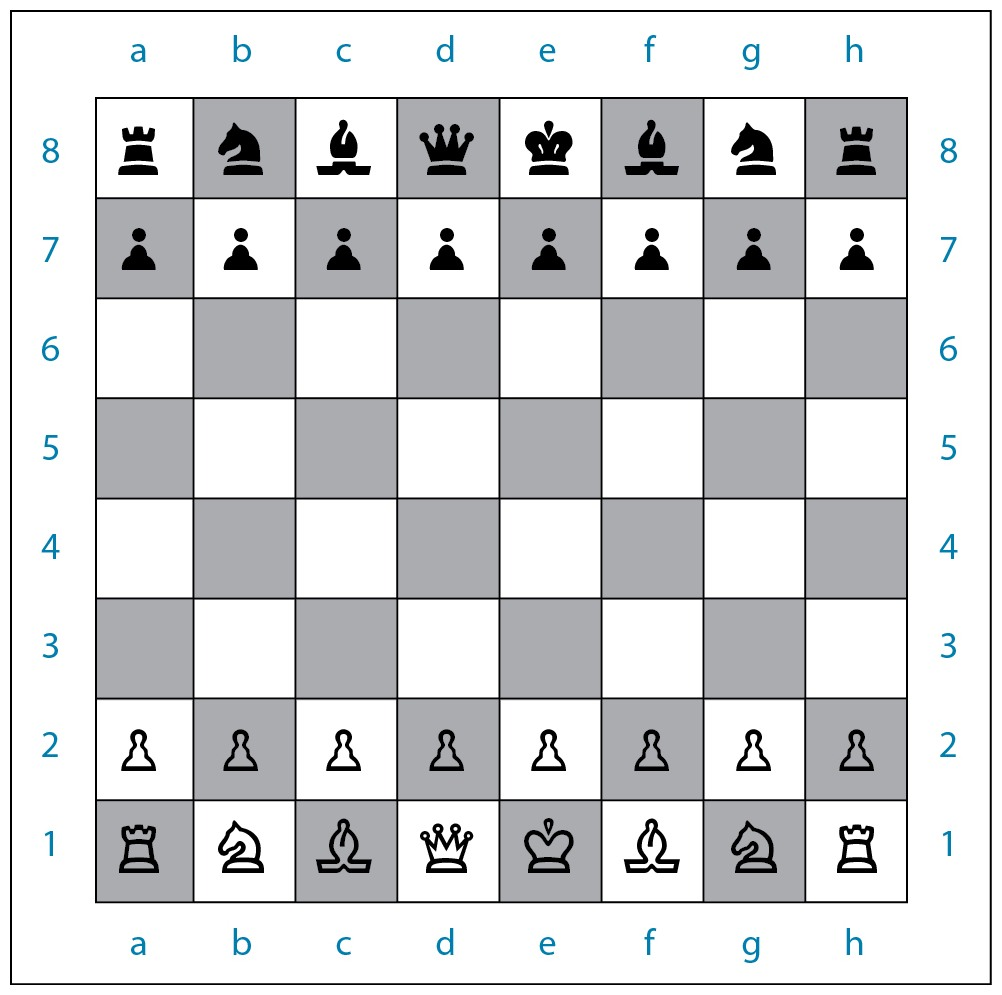
\includegraphics[width=.75\textwidth]{./img/GAMES4_FIG03.08.jpg}
\end{center}
\end{frame}

\begin{frame}[label={sec:orga057086}]{}
\alert{Chess}
\begin{itemize}
\item 400 possible positions (nodes) after each player moves once
\item 9 million after the third move
\item 288 billion after the forth move
\item 40 move game: More possible positions than fundamental particles in the universe
\end{itemize}
\end{frame}
\end{document}